\documentclass[a5paper, 11pt]{scrartcl}

\usepackage{mystyle}
\usepackage[europeanresistors]{circuitikz}
\usepackage{siunitx}

\usepackage{scrlayer-scrpage}
 
\clearpairofpagestyles{}
 
\setkomafont{pageheadfoot}{\sffamily\footnotesize}
\setkomafont{pagination}{}

\ohead{Seite~\pagemark}
\ihead{Tim Hilt}

\KOMAoptions{
  % chapterprefix=true,
  headsepline=true,
}

\title{Formelsammlung Elektronik}
\author{Tim Hilt}

\begin{document}

\maketitle

\section{Grundlagen und Wiederholung}

\subsection{Übertragungsfunktion}
\begin{align*}
  F = \frac{U_a}{U_e} = \frac{\text{Widerstände parallel zum Ausgang}}{\text{Widerstände parallel zum Eingang}}
\end{align*}

\mybfcol{Bei Berechnung zweier, paralleler Widerstände \(R_1\) und \(R_2\):}

\begin{align*}
  R_1 || R_2 = \frac{R_1 \cdot R_2}{R_1 + R_2}
\end{align*}

Leistung: \dotfill \(P = \quad \frac{U^2}{R} \quad = \quad U \cdot \frac{U}{R} \quad = \quad U \cdot I\)\\
Zeitkonstante \(\tau\) beim \mybfcol{Kondensator}: \dotfill \(\tau = R \cdot C\)\\
Zeitkonstante \(\tau\) bei der \mybfcol{Spule}: \dotfill \(\tau = \frac{L}{R}\)\\

\begin{figure}[H]
  \centering
  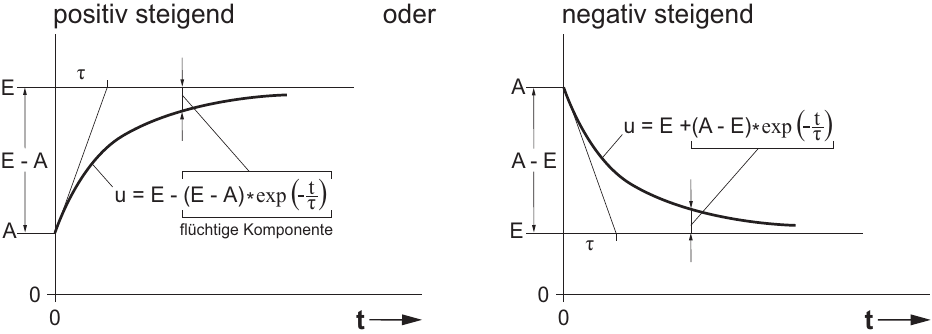
\includegraphics[width=.8\textwidth]{LadekurveKondensator}
  \caption{Ladekurven Kondensator}
\end{figure}

\begin{center}
\begin{tabular}{ll}
  \toprule
  \(t=\tau\) & 63\% von\ \(|A-E|\)\\
  \(t=2\tau\) & 86\% von\ \(|A-E|\)\\
  \(t=5\tau\) & 99\% von\ \(|A-E|\)\\
  \bottomrule
\end{tabular}
\end{center}


\end{document}


%%% Local Variables:
%%% mode: latex
%%% TeX-master: t
%%% End:
